\documentclass[11pt]{article}
\title{MATH 222 Assignment 1}
\author{Sterling Laird - V00834995}
\date{January 24, 2019}

\usepackage{enumitem}
\usepackage{amsmath}
\usepackage{amssymb}
\usepackage {tikz}

\definecolor {myblue}{cmyk}{0.96,0,0,0}

\begin{document}

\maketitle
\pagebreak

\begin{enumerate}[]
    \item
    	Let $n_2$ and $n_2$ be the number of vertices in $G$ of degree 2 and 3 respectively.\\
    	We know that the sum of the degrees of all vertices is twice the number of edges so: \\
    	\begin{gather}
			\sum_{v \in V}deg(v)=2|E| \nonumber \\
			5\cdot 11 + 4\cdot 14 + 3n_3 +2n_2 = 2\cdot 78 \nonumber \\
			3n_3 +2n_2 = 45	
   		\end{gather}
   		We can also sum the total number of vertices:
 	 	\begin{gather}
			11+14+n_3+n_2 = 45 \nonumber \\
			n_2 = 20-n_3
	    \end{gather}
	    Using (1) and (2) we get:
	    \begin{gather}
			3n_3+2(20-n_3)=45  \nonumber \\
 		   	n_3 = 5  \nonumber
		\end{gather}
    	$\therefore$ There are 5 vertices in $G$ with degree 3.
    \item 
    	Since $K_n$ is a complete graph, all vertices are adjacent to all other vertices so a path of length $p$ is isomorphic to any order $p$ subgraph of $K_n$, provided $n \geq p $.\\
    	Since there are $n \choose p$ order $p$ sub-graphs of $K_n$, there will be ${7 \choose 4} = 35$  sub-graphs of $K_7$ that are isomorphic to $P_4$. 
    \item
   		Assume the graph $G$ is not connected.\\
    	Therefore there is at least 2 distinct connected subgraphs $G_1, G_2$ of order $n_1, n_2$.\\
    	It follows that $\forall v \in G_1, deg(v) \leq n_1 -1$ and $\forall v \in G_2, deg(v) \leq n_2 -1$.\\
    	If we choose vertices $x \in G_1$ and $y \in G_2$ then:
    	\begin{gather}
			deg(x) + deg(y) \geq 17  \nonumber \\
			n_1-1 + n_2-1 \geq 17 \nonumber \\
			n_1 + n_2-2 \geq 17 \nonumber \\
			18-2 \geq 17 \nonumber \\
			16 \geq 17
    	\end{gather}
    	But $16 \leq 17$, so (3) is a contradiction.\\
    	$\therefore G$ must be connected.\\
    \item
		\begin{enumerate}[label=\alph*)]
    		\item
   		 		Trivially for $v=\{1\}$ the only $u$ s.t. $v\cup u=S$ is the complete set S and $S\setminus\{1\}$.\\
    			$\therefore deg(\{1\})=2$
    		\item
    			More generally for $v=$a subset of $S$, $v$ is adjacent to all $u=S\setminus w$ $\forall w \subseteq S$.\\
    			Therefore $v$ is adjacent to $2^{|v|}$ vertices when $v\neq S$ and $2^{|v|} -1$ vertices when $v=S$. This is to stop the self loop on $v$ when $v=S$ so that $G$ remains a graph. \\
    			$\therefore deg(\{1,2\}) = 2^2 = 4$
    		\item
    			Since:
    			\begin{gather}
					\sum_{v\in V}deg(v) = 2|E|
    			\end{gather}
    			And because there are $|S| \choose i$ with the same degree $\forall i \in \mathbb{N}$ where $i\leq |S|$:
   			 	\begin{gather}
					\sum_{v\in V}deg(v) = (\sum_{i=0}^{|S|-1} {|S| \choose i}\cdot 2^i) + 2^{|v|} -1
    			\end{gather}
    			Using (4) and (5):
    			\begin{gather}
					1+12+60+160+240+192+63=2|E| \nonumber \\
					|E| = 364 \nonumber
    			\end{gather}
		\end{enumerate}
    \item
		\begin{enumerate}[label=\alph*)]
    		\item 
    			A bipartite graph $G$ on 5 vertices must have one partition that contains 3 vertices that are not adjacent.\\
    			Since the 3 vertices on that partition are not adjacent, $\overline{G}$ will have those 3 vertices be all adjacent.\\
    			Since these 3 vertices are adjacent in $\overline{G}$, for $\overline{G}$ to be bipartite, 2 of these vertices will be in the same partition, but since all 3 are adjacent, there will be an edge within the partition.\\
    			$\therefore$ There cannot be a graph G on 5 vertices s.t. $G$ and $\overline{G}$ are both bipartite.
    		\item
    			Because the complement of $G$ contains all edges in $K_n$ that are not in $E(G)$: 
    			\begin{gather}
					|E(G)| = \frac{|E(K_n)|}{2} \nonumber \\
					|E(G)| = \frac{n(n-1)}{4}
    			\end{gather}
    			Since $|E(G)|$ must be an integer, from (6) we can see that $n(n-1)$ must be divisible by 4.\\
    			It can easily be seen that this is only possible when either $n=4k$ or $n-1=4k  \iff n=4k+1$ for some positive integer $k$.
		\end{enumerate}
    \item			
	As $G$ is a connected graph, and $H$ is not, $G$ and $H$ cannot be isomorphic.\\
    	\begin{center}
    		$G$\\
    		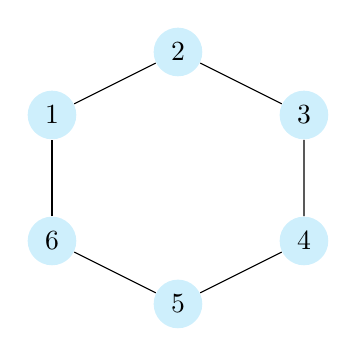
\begin{tikzpicture}
			[scale=.8,auto, every node/.style={circle,fill=myblue!20}]
			\node (1) at (1,1)  {1};
			\node (2) at (3,2)  {2};
			\node (3) at (5,1)  {3};
			\node (4) at (5,-1)  {4};
			\node (5) at (3,-2)  {5};
			\node (6) at (1,-1)  {6};
			
			\foreach \a/\b in {1/2,2/3,3/4,4/5,5/6,6/1}
			\draw (\a) -- (\b);
			\end{tikzpicture}
		\end{center}
		\begin{center}
			$H$\\
			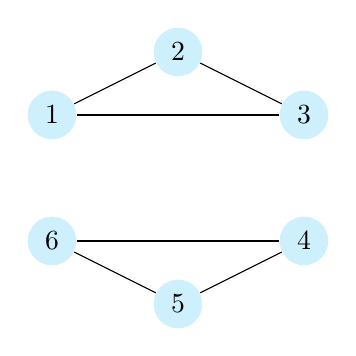
\begin{tikzpicture}
			[scale=.8,auto, every node/.style={circle,fill=myblue!20}]
			\node (1) at (1,1)  {1};
			\node (2) at (3,2)  {2};
			\node (3) at (5,1)  {3};
			\node (4) at (5,-1)  {4};
			\node (5) at (3,-2)  {5};
			\node (6) at (1,-1)  {6};
			
			\foreach \a/\b in {1/2,2/3,3/1,4/5,5/6,6/4}
			\draw (\a) -- (\b);
			\end{tikzpicture}
		\end{center}
		$\therefore$ If $G$ and $H$ have the same number of vertices and the same number of edges and both are 2-regular, $G$ and $H$ are not necessarily isomorphic.
    \item
    	Lets assume that G does not have a cycle. Therefore we can start a path from any vertex and never repeat a vertex without repeating an edge.\\
    	Because every vertex has a degree greater than 2, and $G$ does not have any cycles, there will always be an un-traversed edge to a new vertex at every vertex in the path.\\
    	This implies that the $G$ must be infinite.//
    	Since $G$ is a graph and we consider graphs to be finite, $G$ must contain a cycle if every vertex of $G$ has degree of at least 2.
    \item
		\begin{enumerate}[label=\alph*)]
    		\item
    			Since $K_{m,n}$ is bipartite, for it to have a Hamiltonian cycle each vertex in the cycle must take a path to a node in the other partition before returning to the original vertex in the starting partition. It is clear that this requires that $m=n$ for this to occur because if $m\neq n$ the not all vertices could be in the cycle.\\
    			Since $K_{m,n}$ has an Euler circuit, we know that every vertex has even degree.\\
    			For this to be true both $m$ and $n$ must be even as all vertices in $K_{m,n}$ will have either degree $m$ or $n$.\\
    			$\therefore$ If $K_{m,n}$ has both a Euler circuit and a Hamilton cycle, then $m=n$ and $n$ is even.
    		\item
    			As we can draw a graph that contains a Euler circuit but not a Hamiltonian cycle, the proposition is disproven.\\
    			\begin {center}
    			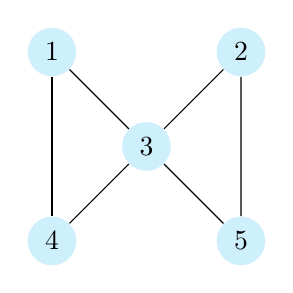
\begin{tikzpicture}
				[scale=.8,auto, every node/.style={circle,fill=myblue!20}]
				\node (1) at (1,4)  {1};
				\node (2) at (4,4)  {2};
				\node (3) at (2.5,2.5)  {3};
				\node (4) at (1,1)  {4};
				\node (5) at (4,1)  {5};
				
				\foreach \a/\b in {1/3,1/4,4/3,2/3,2/5,5/3}
				\draw (\a) -- (\b);
				\end{tikzpicture}
				\end{center}
    		\item
    			The proposition is false as shown in (a), $K_{3,3}$ has a Hamiltonian cycle but no Euler circuit because $m=n$, but $n$ is not even.
		\end{enumerate}
\end{enumerate}

\end{document}